\begin{figure}[H]
\begin{center}
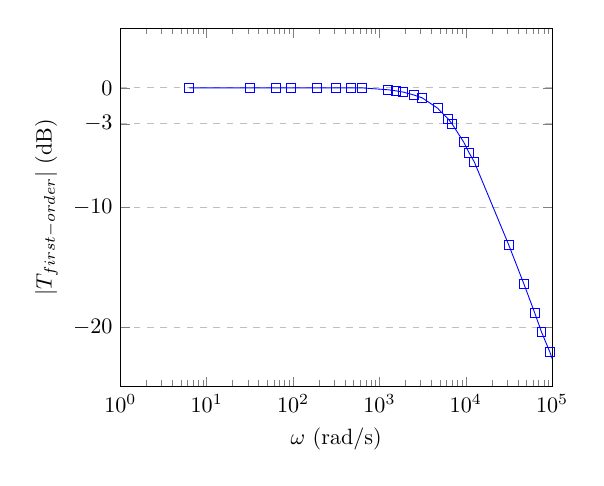
\begin{tikzpicture} [scale=0.8]
\begin{semilogxaxis}[
    title={},
    xlabel={$\omega$ (rad/s)},
    ylabel={$|T_{first-order}|$ (dB)},
    xmin=1, xmax=100000,
    ymin=-25, ymax=5,
    xtick={1,10,100,1000,10000,100000,1000000},
    ytick={0, -3, -10, -20},
    legend pos=north west,
    ymajorgrids=true,
    grid style=dashed,
]
\addplot[
    color=blue,
    mark=square,
    ]
    coordinates {
    (6.28,0)
    (31.42,0)
    (62.83,0)
    (94.25,0)
    (188.5,0)
    (314.16,0)
    (471.24,0)
    (628.32,0)
    (1256.64,-0.156)
    (1570.80,-0.253)
    (1884.96,-0.351)
    (2513.27,-0.596)
    (3141.59,-0.839)
    (4712.39,-1.694)
    (6283.19,-2.615)
    (6945.43,-3.012)
    (9424.78,-4.510)
    (10995.57,-5.465)
    (12566.37,-6.196)
    (31415.93,-13.120)
    (47123.89,-16.393)
    (62831.85,-18.808)
    (75398.22,-20.419)
    (94247.78,-22.099)
    (113097.34,-23.703)
    (125663.71,-24.324)
    };
\end{semilogxaxis}
\end{tikzpicture}
\hspace{1cm}
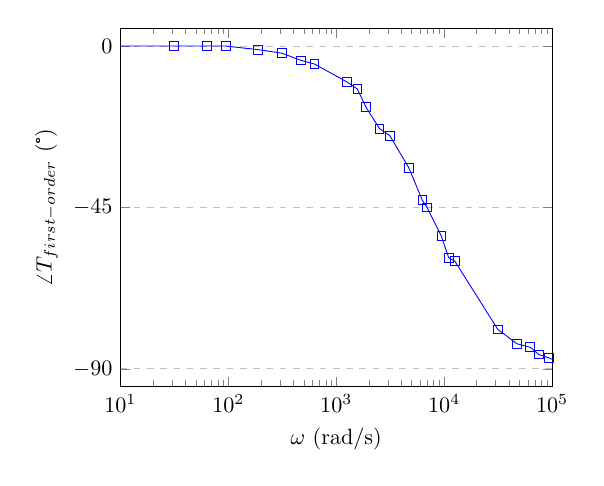
\begin{tikzpicture} [scale=0.8]
\begin{semilogxaxis}[
    title={},
    xlabel={$\omega$ (rad/s)},
    ylabel={$\angle T_{first-order}$ (°)},
    xmin=10, xmax=100000,
    ymin=-95, ymax=5,
    xtick={10,100,1000,10000,100000,1000000},
    ytick={0, -45, -90},
    legend pos=north west,
    ymajorgrids=true,
    grid style=dashed,
]
\addplot[
    color=blue,
    mark=square,
    ]
    coordinates {
    (6.28,0)
    (31.42,0)
    (62.83,0)
    (94.25,0)
    (188.5,-1)
    (314.16,-2)
    (471.24,-4)
    (628.32,-5)
    (1256.64,-10)
    (1570.80,-12)
    (1884.96,-17)
    (2513.27,-23)
    (3141.59,-25)
    (4712.39,-34)
    (6283.19,-43)
    (6945.43,-45)
    (9424.78,-53)
    (10995.57,-59)
    (12566.37,-60)
    (31415.93,-79)
    (47123.89,-83)
    (62831.85,-84)
    (75398.22,-86)
    (94247.78,-87)
    (113097.34,-88)
    (125663.71,-89)
    };
\end{semilogxaxis}
\end{tikzpicture}
\end{center}
\caption{Curvas de bode com os resultados práticos da função de transferência do filtro passa-baixas de 1ª ordem.}
\label{graph:1} 
\end{figure}